\documentclass[,a4paper,12pt,french]{article}

\usepackage[TD]{../../../Style}

% Début du document
%%%%%%%%%%%%%%%%%%%
\begin{document}

\titre{Variations de fonctions}

\begin{multicols*}{2}

\begin{exercice} \label{schemafonctions}
Dresser le tableau de variation des fonctions $f$, $g$ et $h$ définies sur le repère suivant:
\begin{centrer}
\begin{tikzpicture}[scale=\echellepgf]
\begin{axis}[
styleglobal,
width=0.8*\echellepgfinv*\linewidth,
xmin=-0.5, xmax= 8.5,
ymin=-2.5, ymax=3.5,
xtick distance=1,
ytick distance=1,
minor x tick num=1,
minor y tick num=1,
]
\addplot[styleplot,domain=(0:8)] plot {0.5*x-1.5)} node[pos=0.75,above] {$\mathscr C_f$};
\addplot[styleplot,color=DarkRed,densely dashed,domain=(0:8)] plot coordinates{(0,-2) (1,-1) (2,2) (3,3) (5,1) (6,0) (8,-2)} node[pos=0.6,above right] {$\mathscr C_g$};
\addplot[styleplot,densely dotted,color=DarkGreen,domain=(0:8)] plot coordinates{(0,3) (2,2) (3,0) (4,-2) (6,0) (7,2) (8,3)} node[pos=0.1,above right] {$\mathscr C_h$};
\end{axis}
\end{tikzpicture}
\end{centrer}
\end{exercice}

\begin{exercice}
Tracer la représentation graphique d'une fonction définie sur $[-3;5]$ dont le tableau de variations est donné ci-dessous:
\end{exercice}

\begin{exercice}
Fonction croissante. Comparer $f(-1)$ et $f(1)$...
\end{exercice}

\begin{exercice}
On se donne les fonctions $f$ et $g$, représentées sur le repère suivant:
\begin{centrer}
\begin{tikzpicture}[scale=\echellepgf]
\begin{axis}[
styleglobal,
width=0.8*\echellepgfinv*\linewidth,
xmin=-0.5, xmax= 8.5,
ymin=-2.5, ymax=3.5,
xtick distance=1,
ytick distance=1,
minor x tick num=1,
minor y tick num=1,
]
\addplot[styleplot,domain=(0:8)] plot {0.5*x-1.5)} node[pos=0.75,above] {$\mathscr C_f$};
\addplot[styleplot,color=DarkRed,densely dashed,domain=(0:8)] plot coordinates{(0,-2) (1,-1) (2,2) (3,3) (5,1) (6,0) (8,-2)} node[pos=0.6,above right] {$\mathscr C_g$};
\addplot[styleplot,densely dotted,color=DarkGreen,domain=(0:8)] plot coordinates{(0,3) (2,2) (3,0) (4,-2) (6,0) (7,2) (8,3)} node[pos=0.1,above right] {$\mathscr C_h$};
\end{axis}
\end{tikzpicture}
\end{centrer}
\begin{itemize}
\item Donner le maximum de $f$
\item Donner le minimum de $g$ et les antécédents associés.
\item Donner le max de $g$ sur l'intervalle ...
\end{itemize}
\end{exercice}

\begin{exercice}
Pareil avec tableau de variations
\end{exercice}

\begin{exercice}[*] \
\begin{enumerate}
\item Démontrer que la fonction $f:x \mapsto 2x$ est croissante. On se donnera $x,y \in \R$ avec $x<y$ et on montrera que $f(x)<f(y)$.
\item Plus généralement, montrer qu'une fonction affine $f:x \mapsto ax+b$ est croissante si $a>0$, décroissante si $a<0$.
\item Soit $g:x \mapsto x^2$. Dresser le tableau de variations de $g$ sur $\R$, à l'aide de la calculatrice.
\item Démontrons que $g$ est croissante sur $[0;+\infty[$. Soient $x,y \geq 0$ tels que $x<y$.
\begin{enumerate}
\item Quel est le signe de $y+x$? de $y-x$?
\item Quel est alors le signe de $(y+x)(y-x)$?
\item Déterminer alors le signe de $f(y)-f(x)$, puis conclure.
\end{enumerate}
\end{enumerate}
\end{exercice}

\begin{exercice}[*]
On se donne une fonction $f$ définie sur $[-5;4]$. On a dressé son tableau de variations et son tableau de signes ci-dessous:
\begin{centrer}
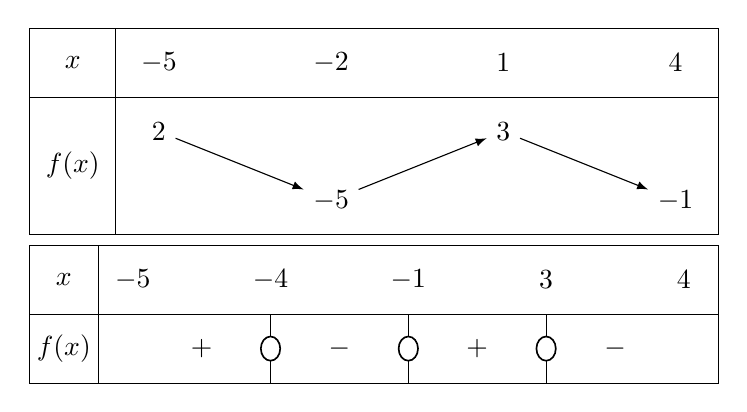
\begin{tikzpicture}[scale=0.875]
% Styles 
\tikzstyle{cadre}=[thin]
\tikzstyle{fleche}=[->,>=latex,thin]
\tikzstyle{nondefini}=[lightgray]
% Dimensions Modifiables
\def\Lrg{5/4}
\def\HtX{1}
\def\HtY{0.5}
% Dimensions Calculées
\def\lignex{-0.5*\HtX}
\def\lignef{-1.5*\HtX}
\def\separateur{-0.5*\Lrg}
% Largeur du tableau
\def\gauche{-1.5*\Lrg}
\def\droite{6.5*\Lrg}
% Hauteur du tableau
\def\haut{0.5*\HtX}
\def\bas{-1.5*\HtX-2*\HtY}
% Ligne de l'abscisse : x
\node at (-1*\Lrg,0) {$x$};
\node at (0*\Lrg,0) {$-5$};
\node at (2*\Lrg,0) {$-2$};
\node at (4*\Lrg,0) {$1$};
\node at (6*\Lrg,0) {$4$};
% Ligne de la fonction : f(x)
\node  at (-1*\Lrg,{-1*\HtX+(-1)*\HtY}) {$f(x)$};
\node (f1) at (0*\Lrg,{-1*\HtX+(0)*\HtY}) {$2$};
\node (f2) at (2*\Lrg,{-1*\HtX+(-2)*\HtY}) {$-5$};
\node (f3) at (4*\Lrg,{-1*\HtX+(0)*\HtY}) {$3$};
\node (f4) at (6*\Lrg,{-1*\HtX+(-2)*\HtY}) {$-1$};
% Flèches
\draw[fleche] (f1) -- (f2);
\draw[fleche] (f2) -- (f3);
\draw[fleche] (f3) -- (f4);
% Encadrement
\draw[cadre] (\separateur,\haut) -- (\separateur,\bas);
\draw[cadre] (\gauche,\haut) rectangle  (\droite,\bas);
\draw[cadre] (\gauche,\lignex) -- (\droite,\lignex);

\begin{scope}[shift= {(-0.38,-3.15)}]
% Styles 
\tikzstyle{cadre}=[thin]
\tikzstyle{fleche}=[->,>=latex,thin]
\tikzstyle{nondefini}=[lightgray]
% Dimensions Modifiables
\def\Lrg{1}
\def\HtX{1}
\def\HtY{0.5}
% Dimensions Calculées
\def\lignex{-0.5*\HtX}
\def\lignef{-1.5*\HtX}
\def\separateur{-0.5*\Lrg}
% Largeur du tableau
\def\gauche{-1.5*\Lrg}
\def\droite{8.5*\Lrg}
% Hauteur du tableau
\def\haut{0.5*\HtX}
\def\bas{-2.5*\HtX-2*\HtY}
% Ligne de l'abscisse : x
\node at (-1*\Lrg,0) {$x$};
\node at (0*\Lrg,0) {$-5$};
\node at (2*\Lrg,0) {$-4$};
\node at (4*\Lrg,0) {$-1$};
\node at (6*\Lrg,0) {$3$};
\node at (8*\Lrg,0) {$4$};
% Ligne de la dérivée : f'(x)
\node at (-1*\Lrg,-1*\HtX) {$f(x)$};
\node at (0*\Lrg,-1*\HtX) {$ $};
\node at (1*\Lrg,-1*\HtX) {$+$};
\draw[cadre] (2*\Lrg,-0.5*\HtX) -- (2*\Lrg,-1.5*\HtX) node[pos=0.5,line width=0.6pt,draw=black,circle,minimum size=7pt,fill=white,inner sep=2pt,yscale=1.25] {};
\node at (3*\Lrg,-1*\HtX) {$-$};
\draw[cadre] (4*\Lrg,-0.5*\HtX) -- (4*\Lrg,-1.5*\HtX) node[pos=0.5,line width=0.6pt,draw=black,circle,minimum size=7pt,fill=white,inner sep=2pt,yscale=1.25] {};
\node at (5*\Lrg,-1*\HtX) {$+$};
\draw[cadre] (6*\Lrg,-0.5*\HtX) -- (6*\Lrg,-1.5*\HtX) node[pos=0.5,line width=0.6pt,draw=black,circle,minimum size=7pt,fill=white,inner sep=2pt,yscale=1.25] {};
\node at (7*\Lrg,-1*\HtX) {$-$};
\node at (8*\Lrg,-1*\HtX) {$ $};
% Ligne de la fonction : f(x)
% Encadrement
\draw[cadre] (\separateur,\haut) -- (\separateur, \lignef);
\draw[cadre] (\gauche,\haut) rectangle  (\droite, \lignef);
\draw[cadre] (\gauche,\lignex) -- (\droite,\lignex);
\end{scope}
\end{tikzpicture}
\end{centrer}
\noindent Tracer dans un repère une courbe représentative potentielle de $f$.
\end{exercice}

\newpage

\end{multicols*}

\end{document}
